\documentclass[a4paper]{ltjsarticle}
\usepackage[top=25mm, bottom=25mm, left=20mm, right=20mm]{geometry}

% 画像
\usepackage[dvipdfmx]{graphicx}
\usepackage{ascmac}
\usepackage{array}
% 表
\usepackage{booktabs}
\usepackage{enumerate}

% 数式
\usepackage{amsmath}
\usepackage{amssymb}
\usepackage{amsfonts}
\usepackage{float}

% ベクトル
\usepackage{bm}
% コード
\usepackage{listings,jvlisting}
% コードの色
\usepackage{color}
\definecolor{OliveGreen}{rgb}{0.0,0.6,0.0}
\definecolor{Orenge}{rgb}{0.89,0.55,0}
\definecolor{SkyBlue}{rgb}{0.28,0.28,0.95}
% ここからコードの表示に関する設定
\lstset{
  basicstyle={\ttfamily},
  identifierstyle={\small},
  commentstyle={\small\itshape},
  keywordstyle={\small\bfseries},
  ndkeywordstyle={\small},
  stringstyle={\small\ttfamily},
  frame= single,
  breaklines=true,
  columns=[l]{fullflexible},
  numbers=none,
  xrightmargin=0.3cm,
  xleftmargin=0.2cm,
  numberstyle={\scriptsize},
  stepnumber=1,
  keepspaces=true,
  keywordstyle={\color{SkyBlue}},
  commentstyle={\color{OliveGreen}},
  stringstyle=\color{Orenge},
  showstringspaces=false
}
\renewcommand{\lstlistingname}{Code}

\newcommand{\E}[1]{\times10^{#1}}
\usepackage{caption}
\usepackage{subcaption}


\usepackage{hyperref}
\usepackage[most]{tcolorbox}


\title{人工知能 期末レポート 課題10}
\author{03240414  小松麟太郎}
\date{\today}


\begin{document}

\maketitle

\section{はじめに}
本課題では大規模言語モデル（LLM）に，新しいメタヒューリスティクスアルゴリズムを提案させる実験を行った．まず，LLMに既存のメタヒューリスティクスをいくつか提示させ，それぞれについて特徴や重要な要素を挙げさせた．その後，それらのメタヒューリスティクスを組み合わせたり改良したりした新しいアルゴリズムを提案させた．最後にLLMが提案したアルゴリズムについて実際にプログラムを実行させて，正しく機能するかの確認，既存のメタヒューリスティクスと性能を比較などをした．使用したLLMのモデルは ChatGPT-4oである．回答はすべてLatexのコードとして出力させた．

\section{課題1}
まず最初にLLMにメタヒューリスティクスを6つ挙げさせ，その詳細について説明させた．このとき，PSOやACOなどの群知能を用いたアルゴリズムに限定させるようにした．用いたプロンプトとそれに対するLLMの回答は次の通り．\\
\textbf{プロンプト}
\begin{tcolorbox}[arc=4mm, enhanced, borderline={0.5mm}{0mm}{black}, breakable, colback = white]
群知能を用いたメタヒューリスティクスの例を6つ挙げ, その詳細について説明して
\end{tcolorbox}
\noindent\textbf{LLMの回答}
\begin{tcolorbox}[arc=6mm, enhanced, borderline={0.5mm}{0mm}{black}, breakable, colback = white]
    \textbf{ 群知能を用いたメタヒューリスティクスの例}

    \vspace{10pt}
    
    \noindent \textbf{1. アリコロニー最適化（Ant Colony Optimization, ACO）}\\
    アリのフェロモン経路形成を模倣し、最適解を探索するアルゴリズムである。\\
    ・アリはランダムに道を探索し、フェロモンを残す。\\
    ・短い経路ほどフェロモンが濃くなり、他のアリが優先して通る。\\
    ・時間とともに最適な経路が強化される。\\
    適用例: 経路最適化（巡回セールスマン問題）、ネットワークルーティング。
    
    \vspace{10pt}
    
    \noindent \textbf{2. 粒子群最適化（Particle Swarm Optimization, PSO）}\\
    鳥や魚の群れの行動を模倣し、最適解を探索するアルゴリズムである。\\
    ・各粒子は自身の最良解（pBest）と群全体の最良解（gBest）を記憶。\\
    ・速度と位置を更新しながら最適解に収束する。\\
    適用例: ニューラルネットワーク学習、連続関数の最適化、ロボットの経路計画。
    
    \vspace{10pt}
    
    \noindent \textbf{3. 人工蜂コロニー（Artificial Bee Colony, ABC）}\\
    ミツバチの採餌行動を模倣したアルゴリズムで、探索と搾取のバランスを取る。\\
    ・働き蜂が蜜源を探索し、質に応じて採餌行動を変える。\\
    ・優れた蜜源ほど探索が強化されるが、局所解に陥らないよう分散探索を行う。\\
    適用例: 機械学習の最適化、スケジューリング問題。
    
    \vspace{10pt}
    
    \noindent \textbf{4. 狼群アルゴリズム（Grey Wolf Optimizer, GWO）}\\
    オオカミの群れの捕食戦略を模倣した最適化手法である。\\
    ・群れにはリーダー（アルファ）、副リーダー（ベータ）、追従者（デルタ）、一般個体（オメガ）がいる。\\
    ・アルファが最適解を示し、他のオオカミが適応しながら探索を行う。\\
    適用例: 画像処理、機械学習のパラメータ最適化。
    
    \vspace{10pt}
    
    \noindent \textbf{5. コウモリアルゴリズム（Bat Algorithm, BA）}\\
    コウモリのエコーロケーション（超音波による探索）を模倣した最適化手法。\\
    ・コウモリはランダムに飛びながら最適解を探索する。\\
    ・周波数や音量の調整により探索と収束のバランスを取る。\\
    適用例: 工学的最適化、パターン認識。
    
    \vspace{10pt}
    
    \noindent \textbf{6. カッコウ探索アルゴリズム（Cuckoo Search, CS）}\\
    カッコウの托卵戦略を模倣し、新しい解（卵）を探索するアルゴリズム。\\
    ・確率的に卵が排除されることで、探索が洗練される。\\
    ・レヴィ飛行（Levy Flight）を用いて広範囲な探索を実現。\\
    適用例: 設計最適化、生物学的データ解析。
\end{tcolorbox}    
\section{課題2}
課題2では課題1でLLMに挙げさせた6つのアルゴリズムについて，重要な特徴と探索性能に影響を与える要素について，それぞれ説明させた．用いたプロンプトとLLMの回答は次の通り．LLMの回答には，致命的な間違いなどは特になかった．\\\\\noindent
\textbf{プロンプト}
\begin{tcolorbox}[arc=4mm, enhanced, borderline={0.5mm}{0mm}{black}, breakable, colback = white]
上記のアルゴリズムについて，重要な特徴や探索性能に影響を与える要素についてそれぞれ説明して.
\end{tcolorbox}
\noindent\textbf{LLMの回答}
\begin{tcolorbox}[arc=6mm, enhanced, borderline={0.5mm}{0mm}{black}, breakable, colback = white]

    \textbf{群知能を用いたメタヒューリスティクスの特徴と探索性能に影響を与える要素}

    \vspace{10pt}
    
    \noindent \textbf{1. アリコロニー最適化（Ant Colony Optimization, ACO）}\\
    \textbf{特徴:} \\
    ・経路探索に適しており、局所最適解を回避するためのフェロモン蒸発機構を持つ。\\
    ・適応的に探索を行うため、大規模な組合せ最適化問題に適用可能。\\
    \textbf{探索性能に影響を与える要素:} \\
    ・フェロモンの蒸発率: 低すぎると局所解に陥りやすく、高すぎると探索が安定しない。\\
    ・情報拡散率: 最適解の強調度合いが探索のバランスに影響を与える。
    
    \vspace{10pt}
    
    \noindent \textbf{2. 粒子群最適化（Particle Swarm Optimization, PSO）}\\
    \textbf{特徴:} \\
    ・収束が高速であり、連続最適化問題に適している。\\
    ・群れ全体の情報共有を利用して、探索を効率化する。\\
    \textbf{探索性能に影響を与える要素:} \\
    ・慣性係数: 大きいとグローバル探索、小さいとローカル探索が強化される。\\
    ・学習係数（個体と群れ）: 個体の探索の自由度と、群れ全体の収束バランスを決定する。
    
    \vspace{10pt}
    
    \noindent \textbf{3. 人工蜂コロニー（Artificial Bee Colony, ABC）}\\
    \textbf{特徴:} \\
    ・探索（探索蜂）と搾取（観察蜂）のバランスを調整する仕組みを持つ。\\
    ・局所探索を強化するための解の更新戦略がある。\\
    \textbf{探索性能に影響を与える要素:} \\
    ・探索蜂と観察蜂の割合: 局所探索とグローバル探索のバランスに影響。\\
    ・食糧源の選択確率: 優れた解への収束速度を決定。
    
    \vspace{10pt}
    
    \noindent \textbf{4. 狼群アルゴリズム（Grey Wolf Optimizer, GWO）}\\
    \textbf{特徴:} \\
    ・アルファ、ベータ、デルタ、オメガの階層構造を持ち、多様な探索を実現。\\
    ・探索段階と収束段階のバランスが比較的良い。\\
    \textbf{探索性能に影響を与える要素:} \\
    ・パラメータ $a$ の減少速度: 初期の探索能力と最終的な収束速度を決定。\\
    ・アルファ・ベータ・デルタの影響度: 群れのリーダーがどの程度解を主導するか。
    
    \vspace{10pt}
    
    \noindent \textbf{5. コウモリアルゴリズム（Bat Algorithm, BA）}\\
    \textbf{特徴:} \\
    ・エコーロケーションを模倣し、周波数と音量の調整により適応的な探索を行う。\\
    ・探索の多様性と収束性のバランスを取りながら進化する。\\
    \textbf{探索性能に影響を与える要素:} \\
    ・超音波の周波数範囲: グローバル探索とローカル探索のバランスを決定。\\
    ・音量の変化率: 収束速度と解の多様性に影響。
    
    \vspace{10pt}
    
    \noindent \textbf{6. カッコウ探索アルゴリズム（Cuckoo Search, CS）}\\
    \textbf{特徴:} \\
    ・レヴィ飛行を利用して広範囲な探索が可能。\\
    ・単純な構造ながら強力な探索性能を持つ。\\
    \textbf{探索性能に影響を与える要素:} \\
    ・レヴィ飛行のパラメータ: 解の探索範囲を決定し、局所解への陥りにくさに影響。\\
    ・巣の更新率: 新しい解を導入する頻度を決定し、探索の多様性に関わる。
    
\end{tcolorbox}

\section{課題3}
課題3では，課題1，2を踏まえて，それらのアルゴリズムを改良したり組み合わせたりして， 新しいハイブリッドのアルゴリズムをLLMに考案させるということをした．扱う問題は連続最適化問題としたとした．アルゴリズムの条件として，局所最適解に陥りにくい，種の多様性を維持しやすい，の2つを課した．用いたプロンプトとLLMの回答は次のようになった．\\\quad
LLMは, PSO（Particle Swarm Optimization），CS(Cuckoo Search)，GWO（Gray Wolf Optimizer）の3つのメタヒューリスティクスを組み合わせて， ASGCO (Adaptive Swarm-Guided Cuckoo Optimization) という新しいアルゴリズムを提示した．ASGCOでは，PSOの更新式で位置を更新した後GWOの更新式で位置を更新し，さらにCSのレヴィ飛行を使ってさらに位置を更新していることが分かる．\\
次にLLMにこのアルゴリズムのPythonコードを出力させた．このとき，LLMは世代の更新部分にGWOの要素を入れず，PSOによる更新と，レヴィ飛行の部分だけを書いたコードを出力した．その後もう一度出力させるとGWOの更新部分が含まれたPythonコードが出力された．
\\\noindent
\textbf{プロンプト}
\begin{tcolorbox}[arc=6mm, enhanced, borderline={0.5mm}{0mm}{black}, breakable, colback = white]
    組み合わせ最適化問題を解きたい．前問の特徴を踏まえたうえで，上記のアルゴリズムを改善したり，2，3個組み合わせたりして，多様性が維持でき，かつ局所最適解に陥りにくい，新しいメタヒューリスティクスのアルゴリズムを自分で考え，その疑似コードを示せ
\end{tcolorbox}
\noindent
\textbf{LLMの回答}
\begin{tcolorbox}[arc=6mm, enhanced, borderline={0.5mm}{0mm}{black}, breakable, colback = white]
    \textbf{ Adaptive Swarm-Guided Cuckoo Optimization (ASGCO)}

    \vspace{10pt}

    \noindent \textbf{アルゴリズムの概要}\\
    ASGCOは、以下の3つのアルゴリズムを組み合わせることで、局所最適解に陥りにくく、多様性を維持することを目的とする。  
    \begin{itemize}
        \item \textbf{粒子群最適化（PSO）}: 高速な収束性を活かし、最適解を効率的に探索する。
        \item \textbf{カッコウ探索（CS）}: レヴィ飛行を利用し、広範囲の探索を可能にする。
        \item \textbf{狼群アルゴリズム（GWO）}: 群れのリーダー戦略を導入し、多様性を維持する。
    \end{itemize}

    \vspace{10pt}

    \noindent \textbf{アルゴリズムの流れ}
    \begin{enumerate}
        \item \textbf{初期化}:
        \begin{itemize}
            \item PSOの粒子群をランダムに初期化し、位置と速度を設定する。
            \item 各粒子の最良解（$pBest$）と全体の最良解（$gBest$）を記録する。
            \item 狼群アルゴリズムに基づき、粒子を「アルファ」「ベータ」「オメガ」に分類する。
        \end{itemize}
        
        \item \textbf{探索ステップ}:
        \begin{itemize}
            \item PSOの更新式を適用し、粒子の移動を行う。
            \item 確率 $P_{levy}$ でランダムに粒子を選び、カッコウ探索（CS）のレヴィ飛行を適用し、大域的な探索を行う。
            \item 群れのリーダー（GWOのアルファ）が探索の方向を決定し、他の粒子がそれに従う。
        \end{itemize}
        
        \item \textbf{適応的なパラメータ調整}:
        \begin{itemize}
            \item 局所最適解に陥った粒子の速度をリセットし、大域探索へシフトする。
            \item レヴィ飛行の確率 $P_{levy}$ を進行状況に応じて調整し、探索の多様性を維持する。
        \end{itemize}
        
        \item \textbf{収束判定}:
        \begin{itemize}
            \item 規定の反復回数に達するか、最適解が収束すれば終了する。
        \end{itemize}
    \end{enumerate}
    \vspace{10pt}

    \noindent \textbf{疑似コード}\\
    \begin{lstlisting}[frame = tb]
アルゴリズム: ASGCO（適応型群知能誘導カッコウ最適化）

入力:
    - 目的関数 f(x)
    - 粒子数 N
    - 最大反復回数 MaxIter
    - PSO の慣性係数 w, 学習係数 c1, c2
    - CS のレヴィ飛行確率 P_levy
    - GWO のリーダー階層

初期化:
    1. 各粒子の位置 x_i をランダムに初期化
    2. 各粒子の速度 v_i をランダムに初期化
    3. 各粒子の最良解 pBest_i を自身の初期位置に設定
    4. 全体の最良解 gBest を群全体の最良の pBest で初期化
    5. 群れを GWO のアルファ (α), ベータ (β), デルタ(δ) オメガ (ω) に分類

探索ステップ:
    6. for iter = 1 to MaxIter do
        7. for 各粒子 i do
            8. 標準 PSO に基づいて速度を更新:
                v_i = w * v_i + c1 * rand() * (pBest_i - x_i) + c2 * rand() * (gBest - x_i)
            9. 位置を更新:
                x_i = x_i + v_i
            10. 新しい位置の評価:
                if f(x_i) < f(pBest_i) then
                    pBest_i = x_i
                end if
        11. 群れのアルファ (α), ベータ (β), デルタ(δ) オメガ (ω)を更新 (GWO に基づく)

        12. 一定確率 P_levy でランダムに選ばれた粒子にカッコウ探索 (CS) のレヴィ飛行を適用:
            x_levy = gBest + α * LevyFlight()
            if f(x_levy) < f(gBest) then
                gBest = x_levy
            end if

        13. 局所最適に陥っている粒子に対し、速度をリセットし探索範囲を拡大

        14. 収束条件を満たした場合、終了

出力:
    - 最適解 gBest

    \end{lstlisting}

    \vspace{10pt}
    

    \noindent \textbf{特徴と利点}\\
    ASGCOは、PSOの収束速度、CSの大域探索能力、GWOの多様性維持を組み合わせた新しい最適化手法である。
    \begin{itemize}
        \item 高速な収束と広範囲な探索を両立
        \item 局所最適に陥りにくく、多様性を維持
        \item 適応的なパラメータ調整により探索能力を強化
    \end{itemize}
    
\end{tcolorbox}

\section{LLMの提示したアルゴリズムの評価}
\subsection{評価方法}
実際にLLMが提示した新しいアルゴリズムをPythonで実装し，他の手法との性能比較を行った．性能評価に用いた関数は以下の4つの多峰関数を用いた．いずれの関数も最小値は，$x_i = 0 \quad (i = 1, 2, \cdots)$ のとき $f = 0$ である．
\begin{itemize}
    \item \textbf{問題1 : Ackley関数}
        \begin{align*}
            f(\mathbf{x}) = -20 \exp\left(-0.2 \sqrt{\frac{1}{d} \sum_{i=1}^{d} x_i^2}\right) - \exp\left(\frac{1}{d} \sum_{i=1}^{d} \cos(2 \pi x_i)\right) + 20 + e
        \end{align*}
    \item \textbf{問題2 : Rosenbrock関数}
        \begin{align*}
            f(\mathbf{x}) = \sum_{i=1}^{d} \left[100 (x_{i+1} - x_i^2)^2 + (1 - x_i)^2\right]
        \end{align*}


    \item \textbf{問題3 : Rastrigin関数}
        \begin{align*}
            f(\mathbf{x}) = 10d + \sum_{i=1}^{d} \left[x_i^2 - 10 \cos(2 \pi x_i)\right]
        \end{align*}

    \item \textbf{問題4 : Griewank関数}
        \begin{align*}
            f(\mathbf{x}) = 1 + \frac{1}{4000} \sum_{i=1}^{d} x_i^2 - \prod_{i=1}^{d} \cos\left(\frac{x_i}{\sqrt{i}}\right)
        \end{align*}
\end{itemize}
これらの関数の入力次数はいずれも5とした．また，比較するアルゴリズムには，LLMがASGCOを提案するのに参考にした，CS，GWO．PSOの3つのアルゴリズムを用いた．それぞれのアルゴリズムでは個体数30，世代数100とし，その他のパラメーターは次のようにした．
\begin{itemize}
    \item \textbf{ASGCO}\\
        慣性係数 $w$ = 0.7 ,  学習係数 $c_1 = c_2 = 1.5$, レヴィ飛行確率 $p_l = 0.2$
    \item \textbf{PSO}\\
        慣性係数 $w$ = 0.7 ,  学習係数 $c_1 = c_2 = 1.5$
    \item \textbf{CS}\\
        巣の放棄率 $p_a = 0.25$
\end{itemize}

\begin{figure}[b]
    \centering
    \begin{minipage}{0.49\linewidth}
        \centering
        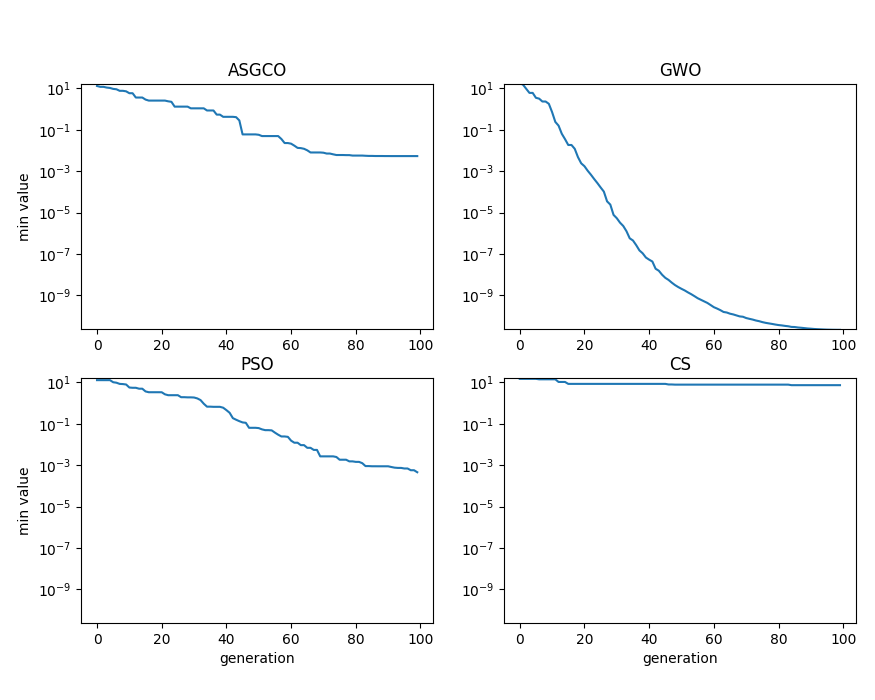
\includegraphics[width = \linewidth]{figure/Ackley.png}
        \caption{Ackley関数}
    \end{minipage}
    \hfill
    \begin{minipage}{0.49\linewidth}
        \centering
        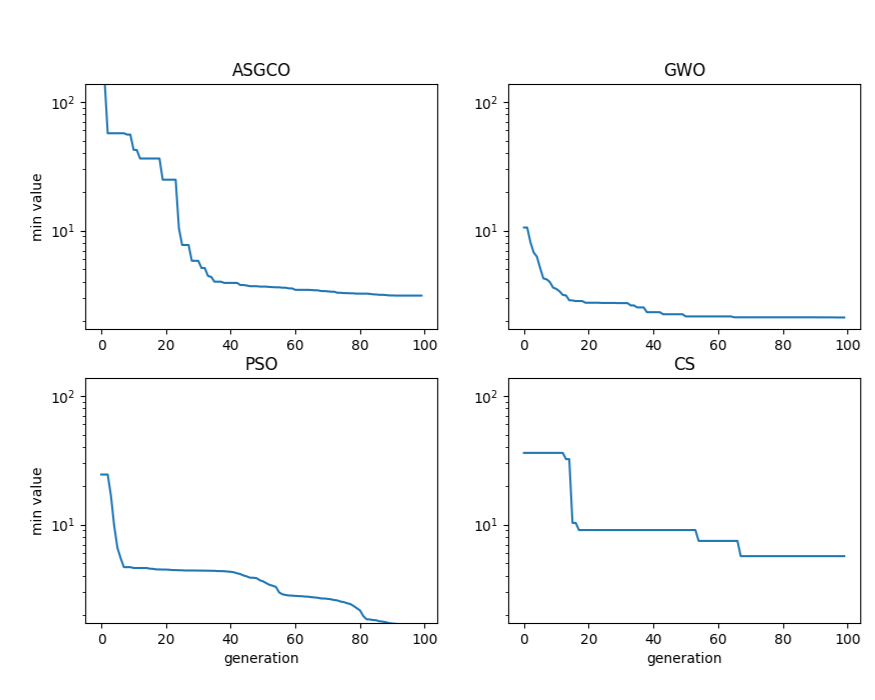
\includegraphics[width = \linewidth]{figure/Rosenbrock.png}
        \caption{Rosenbrock関数}
    \end{minipage}
\end{figure}
\begin{figure}[b]
    \centering
    \begin{minipage}{0.49\linewidth}
        \centering
        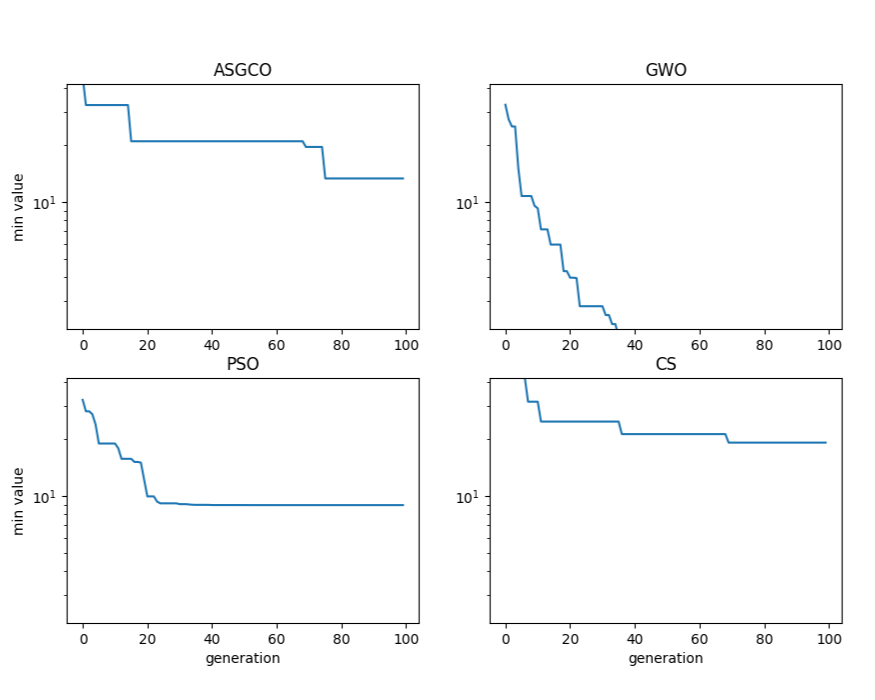
\includegraphics[width = \linewidth]{figure/Rastrigin.png}
        \caption{Rastrigin関数}
    \end{minipage}
    \hfill
    \begin{minipage}{0.49\linewidth}
        \centering
        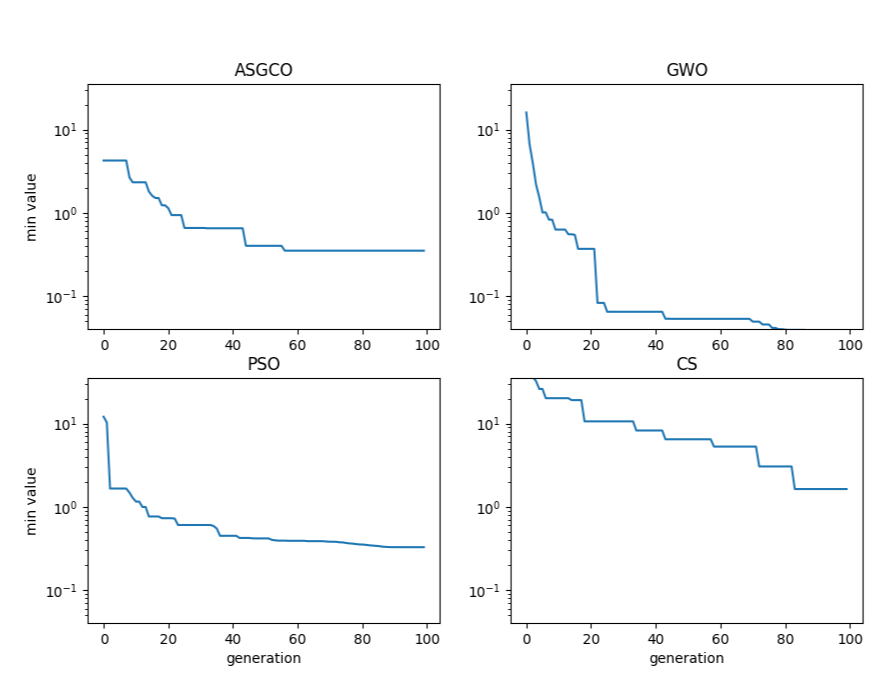
\includegraphics[width = \linewidth]{figure/Griewank.png}
        \caption{Griewank関数}
    \end{minipage}
\end{figure}

\subsection{結果}
図1から4は前節で述べた4つの関数についてそれぞれASGCO, GWO, PSO, CSのアルゴリズムを適用し，最小値を探索した結果である．横軸が世代数，縦軸が探索で得られた関数の最小値を対数で表したものである．図から，Ackley関数，Rastrigin関数，Griewank関数の3つではGWOで最も小さい値が得られ，Rosenbrock関数では，PSOで最も小さい値が得られていることが分かる．ASGCOは，どの関数においてもCSよりも小さい値を得たが，GWOやPSOと比べると，Greiwank関数やRosenbrock関数などの一部でGWOやPSOと同等の値を見つけてはいるが全体としてはPSOやGWOよりも大きな値が得られていることが分かる．したがって，連続最適化の問題に関して，LLMが考案したASGCOは，CSより性能が高く，GWOやPSOよりも性能が劣っていると考えられる．
\section{考察}
本課題では，LLMに既存のメタヒューリスティクスをもとに新しいハイブリッドアルゴリズムを提案させ，その実装と評価を行った．その結果，LLMは既存のメタヒューリスティクスに関する説明を致命的なミスなく行うことができた．また，新たにASGCOというアルゴリズムを提案し，Pythonで実行したところ，実際に最適解の探索を行うことができた．しかし，性能評価の結果，LLMがASGCOを提案する際に参照したGWOやPSOといった既存のアルゴリズムの方が高性能であることが確認された．\\\quad
また，LLMにASGCOの実行可能なPythonコードを出力させた際，初めは疑似コードと異なる内容のコードが生成された．既存のGWOやPSOのコードを出力させた場合には問題なく正確なコードが生成されたことから，LLMは既存のアルゴリズムについては学習データをもとにほぼ正確なコードを出力できるが，新規のアルゴリズムについては正確なコードを出力できるとは限らないことが分かった．そのため，新しいアルゴリズムを実装する際には，LLMが生成したコードを十分に検証する必要がある．\\\quad
新たに考案したASGCOの性能については，PSOやGWOと比較して劣る結果となった．ただし，LLMはPSOやGWOについては学習済みであり，それぞれのアルゴリズムに対するパラメータも最適化されている可能性が高い．一方で，ASGCOは新規のアルゴリズムであるため，パラメータは最適化されておらず，適切なチューニングを行えば，より良い結果が得られる可能性がある．\\\quad
本課題では，LLMが完全なPythonコードを生成することはできなかったものの，使用したモデルはChatGPT-4oであり，最近発表された上位モデルであるo1やo3を用いれば，より高度な思考が可能となり，新規アルゴリズムの実装においてもバグの少ないコードを生成できるかもしれない．仮に正確なコードを出力できなかったとしても，LLMは実用可能なハイブリッドアルゴリズムを考案する能力を有しており，新しいアルゴリズムの設計を行う際の参考として活用する価値があると考えられる．



\end{document}